\section{Local Optimizations}

Local Optimizations never goes away because this is always a piece of what happens even when we 
talk about even more sophiscated types of optimizations.

First we will talk about how to represent the code within a function or procedure, that's using 
something called a flow graph which is made of basic blocks.  Next we will contrast two different 
abstractions for doing local optimizations.




\subsection{Basic Blocks/Flow graphs} 


\subsubsection{Basic Blocks}

A basic block is a sequence of instructions(3-address statements). There are some requirements for basic 
block:

\begin{itemize}
    \item \textbf{Only the first instruction can be reached from outside the blcok.} The reason why this property 
    is useful is that within a basic block, we just march instruction by instruction through the block, 
    this simplies things at least within a basic block.
    \item \textbf{All the statements are executed consecutively if the first one is.}
    \item \textbf{The basic block must be maximal.} i.e., they cannot be made larger without violating conditions. 
\end{itemize}


\subsubsection{Flow graphs}
Flow graph is a graph representation of the procedure. In flow graph, basic blocks are the nodes, and the edge for \(  B_i 
\rightarrow B_j \) stands for a path from node \( B_i \) to node \( B_j \). So how will \(  B_i  \rightarrow B_j \) happen? 
There are two possibilities:

\begin{itemize}
    \item Either first instruction of \(B_j\) is the target of a goto at end of \(B_i\).
    \item \(B_j\) physically follows \(B_i\) which doesn't end in an unconditional goto.
\end{itemize}




% \begin{center}

% \begin{tikzpicture}[auto,
%     node distance = 12mm,
%     start chain = going below,
%     box/.style = {draw,rounded corners,blur shadow,fill=white,
%           on chain,align=center}]
%    \node[box] (b1)    {$x_1\leftarrow0$\\ $y_1\leftarrow0$};      
%    \node[box] (b2)    {$x_2\leftarrow\phi(x_1,x_3)$\\
%    $y_2\leftarrow\phi(y_1,y_3)$\\
%    $(x_2<10)$?};      
%    \node[box] (b3)    {$y_3\leftarrow y_2+x_2$\\ $x_3\leftarrow x_2+1$};  
%    \node[box] (b4)    {print($y_2$)};     
%    \begin{scope}[rounded corners,-latex]
%     \path (b2.-40) edge[bend left=50] (b4.40)
%     (b1) edge (b2) (b2) edge (b3);
%     \draw (b3.230) -- ++(0,-0.3) -| ([xshift=-5mm]b2.west) |-
%     ([yshift=3mm]b2.130) -- (b2.130);
%    \end{scope}
%   \end{tikzpicture}

% \end{center}




\subsubsection{Partitioning into Basic Blocks}

\begin{itemize}
\item Identify the leader of each basic block 
    \begin{itemize}
        \item First instruction
        \item Any target of a jump
        \item Any instruction immediately following a jump
    \end{itemize}

\item Basic block starts at leader and ends at instruction immediately before a leader(or the last instruction).    
\end{itemize}

An example of flow graph is shown below:

\begin{figure}[h]
    \centering
    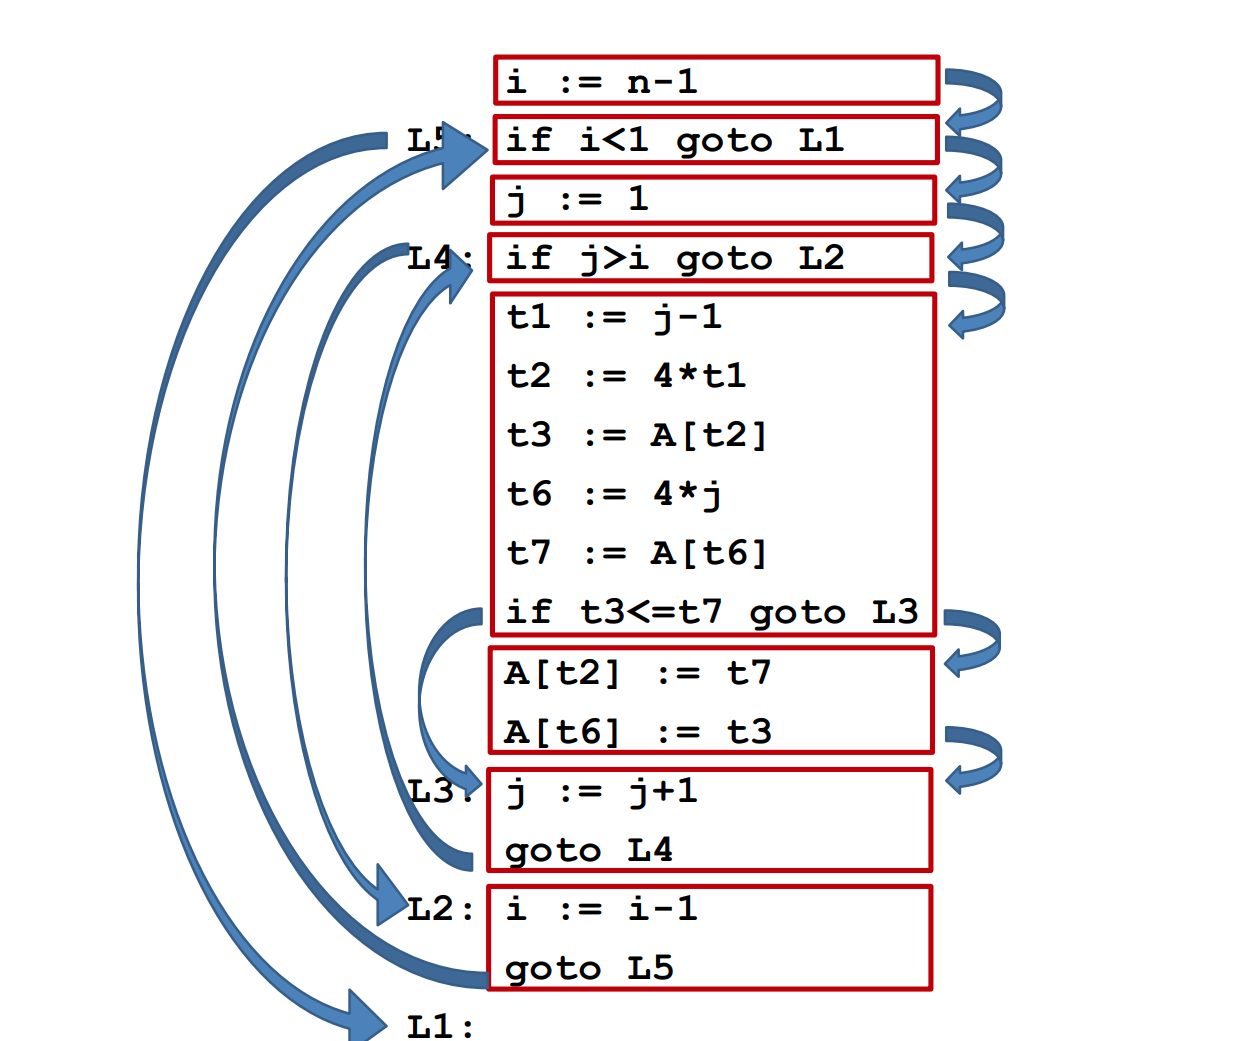
\includegraphics[width=0.5\textwidth]{flowgraph.png}
    \caption{Example of a flow graph}
\end{figure}

\subsubsection{Reachability of Basic Blocks}

There is one thing interesting need to mention here. So the source code is below:

\begin{lstlisting}[language=C,frame=single, caption=An example]
if x { 
    ...
    return;
} else {
    ...
}


\end{lstlisting}


The corresponding flow graph is shown in \ref{fig:fgex}:

\begin{figure}[h]
    \centering
    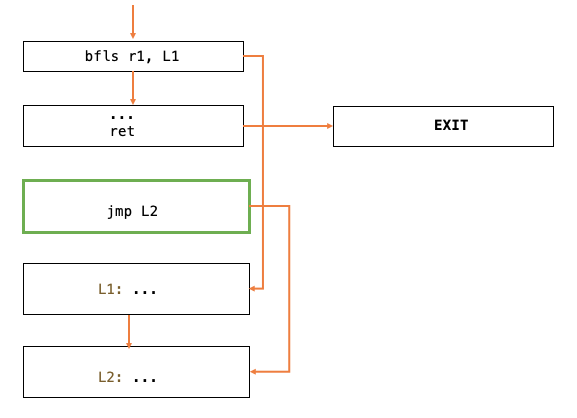
\includegraphics[width=0.5\textwidth]{fgex.png}
    \caption{Example of a flow graph}
    \label{fig:fgex}
\end{figure}


We can see that the box in green is unreachable from the entry. So why is that interesting? Typically, after compiers 
construct the control flow graph, they will go through and remove any unreachable nodes. Just do depth first traversal of the graph
from the entry node and mark all those visited nodes. So unmarked nodes will be deleted. This will help the compiler get a better optimization
result.


So why do these unreachable nodes appear? The anwser is it is not the job of the front-end of the compiler to clean up the unreachable nodes. 



\subsection{Local optimizations}

Local optimizations are those occur \textbf{within the basic blocks}. 


\subsubsection{common subexpression elimination}

There're some types of local optimizations. 
One is called \textbf{common subexpression elimination}. Subexpressions are some arithmetic expressions that occur on the
 right hand of the instructions. Common subexpressions are subexpression that occur many times where the operands have not 
 changed.
 
\begin{lstlisting}[language=C, frame=single,caption=Subexpression example,label=lst:subexp]
a = b + c;
d = b + c;
\end{lstlisting}

In the example \ref{lst:subexp}, \texttt{b + c} is so called coomon subexpression, we could replace the instruction containing 
common subexpression with an assign expression. 


\begin{lstlisting}[language=C, frame=single,caption=code snippet applied common subexpression elimination to \ref{lst:subexp},label=lst:transsubexpr]
    a = b + c;
    d = a
\end{lstlisting}

You may wonder why this kind of redundancy can occure in code? Are we programmers stupid to do so? In fact, 
the redundancy most comes from the stage when compilers  turn your source code. For example, when you use arrays,
you need to do some arithmetic to generate the address of the array element you are accessing. So every time you referece the same
array element, compiler will calculate the same address again. Similarly, if you access offsets within fields. Last example is 
access to parameters in the stack. 


\subsection{Abtraction 1:DAG}

DAG is the acronym for Directed Acyclic Graph. The Directed Acyclic Graph (DAG) is used to represent the 
structure of basic blocks, to visualize the flow of values between basic blocks, and to provide 
optimization techniques in the basic block. DAG is an efficient method for identifying common 
sub-expressions.\footnote{copied from \url{https://wildpartyofficial.com/what-is-dag-in-compiler-construction}}



The parse tree and DAG of the expression \(a + a*(b+c) + (b+c) *d \) is shown in \ref{fig:DAG}.


\begin{figure}[h]
    \centering
    \includegraphics[width=0.5\textwidth]{DAG.png}
    \caption{Example of a DAG}
    \label{fig:DAG}
\end{figure}



In DAG, some of the computation are reused. So we can generate optimizaed code based on DAG.

The optmized code for the DAG\ref{fig:DAG} is: 

\begin{lstlisting}[language=C, frame=single,caption=code ,label=lst:dag]
    t1 = b - c;
    t2 = a * t1;
    t3 = a + t2;
    t4 = t1 * d;
    t5 = t3 + t4;
\end{lstlisting}


\subsubsection{How well do DAGs hold up across statements?}

We have seen that DAGs can be useful in a long arithmetic expression. So how well do DAGs
perform in sequence of instructions?

\begin{lstlisting}[language=C, frame=single,caption=code ,label=lst:dagexpr2]
    a = b + c;
    b = a - d;
    c = b + c;
    d = a - d;
\end{lstlisting}


The corresponding DAG is shown in \ref{fig:DAG2}.
\begin{figure}[h]
    \centering
    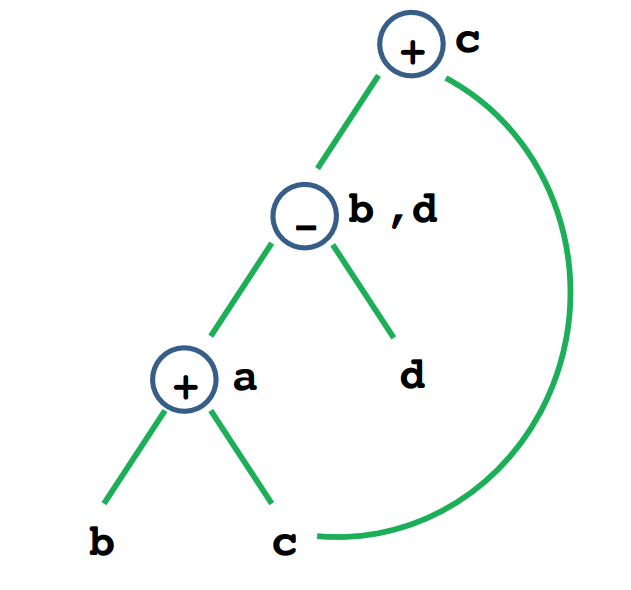
\includegraphics[width=0.5\textwidth]{dag2.png}
    \caption{Example of a DAG}
    \label{fig:DAG2}
\end{figure}

Based on the DAG\ref{fig:DAG2}, one optimizaed code is \ref{lst:dagexprop2}


\begin{lstlisting}[language=C, frame=single,caption=code ,label=lst:dagexprop2]
a = b+c;
d = a-d;
c = d+c;
\end{lstlisting}

\ref{lst:dagexprop2} is not correct. B need to be overwritten but not yet. So if using DAGs, you need to be 
very careful. 

DAGs make sense if you just have one long expression, but once you have sequence of instructions overwriting variables
, DAGs are less appealing because this abstraction doesn't really include the concept of time.




\subsection{Abtraction 2:Value numbering} 

We have seen drawbacks of DAGs. One way to fix the problem is to attach variable name to latest value. Value numbering is 
such abstraction.

The idea behind value numbering is there is a mapping between variables(static) to values(dynamic). So common subexpression means same 
value number.

\subsubsection{Algorithm}


\begin{lstlisting}[language=python, frame=single,caption=code ,label=lst:vna]
Data structure:
    VALUES = Table of
        expression /* [OP, valnum1, valnum2] */
        var /* name of variable currently holding expr */
For each instruction (dst = src1 OP src2) in execution order
    valnum1=var2value(src1); valnum2=var2value(src2)

    IF [OP, valnum1, valnum2] is in VALUES
        v = the index of expression
        Replace instruction with: dst = VALUES[v].var
    ELSE
        Add
            expression = [OP, valnum1, valnum2]
            var = tv
        to VALUES
        v = index of new entry; tv is new temporary for v
        Replace instruction with: tv = VALUES[valnum1].var OP VALUES[valnum2].var
                                dst = tv
    set_var2value (dst, v)  
\end{lstlisting}


\subsubsection{Example}








